\chapter{Methodology}
\label{chap:methodology}

In this chapter we will discuss the methods and guidelines used to create our predictive models and their applications. One can define the task of predicting patient outcomes over time from ICU data is defined as follows. Each ICU patient can be represented by their physiological observations at a given time, such as heart rate, temperature, blood pressure, and others. Since the patient is continuously observed, his representation is an ordered set of multiple discrete time observations.

We then have as input the {\em training set}, which consists of a sequence of observations of the form $<A_t,o>$, where $A_t$ is a vector of values corresponding to physiological parameters associated with a patient at time $t$, and $o$ is the outcome for the patient (i.e., whether or not the patient survived the hospitalization). The training set is used to construct a model that relates features within the sequence of observations to the patient outcome. The {\em test set} consists of a sequence of observations $<A_t,?>$ for which only the physiological parameters for the patient until time $t$ are available, while the corresponding patient outcome is unknown. The model learned from the training set is used to produce predictions of the outcome for patients in the test set. 

The full set of data is split into 5 equally large stratified fold, used to perform a 5-fold cross validation. Each fold is divided in training and test set. Early stopping \citep{prechelt1998automatic} was also applied, so the training set is divided itself in the actual training set, which is used to build the model, and a validation set, used to prevent the neural network from overfitting.

The task of predicting patients outcomes in the ICU has two important requirements:
\begin{itemize}
\item It is a domain-specific problem, i.e., a prediction model learned from a sub-population (or ICU domain) is likely to fail when tested against data from other population~\citep{longi}. Feature transferability is thus an appealing way to provide robustness to prediction models.
\item It is a time-sensitive problem, i.e., accurately predicting patient outcomes as early as possible may lead to earlier diagnosis and more effective therapy.
\end{itemize}

We divide this chapter in two sections. The first shall explicit our methods to achieve the best mortality prediction as possible through a  model, which is built from multi-domain ICU time-series data and is designed to provide dynamically-updated estimates of patient mortality, while the second section will show some practical applications of those models.

\section{Mortality Prediction}

Here we discuss how to manipulate the patient data into a format that can be dynamically consumed by a model, along with the main blocks that constructs this model. We also present our novel neural layer and explain how to apply domain adaptation to help solve the multi-distribution and generalization problem.

Our goal is to analyze patient data at each moment and evaluate the probability of this patient not surviving the treatment, simulating a real time medical expert with full attention to each patient. In order to do so, we need a well defined data structure that consists of fixed time steps and a invariable set of patient's signs at each time step.

\subsection{Data and Domains}

We use the publicly available dataset of multivariate clinical time-series of 4,000 patients from the PhysioNet 2012 challenge~\citep{silva}. The data for each patient includes age, gender, height, weight and 37 time-stamped physiological parameters measured during the first 48 hours of ICU stay. All those parameters are listed in Table \ref{tab:physionet}. Patient outcomes, including mortality, are available. Note that some of those features are measured a lot more frequently than others, as each feature as its own measurement difficulty. For instance, it is quite simple to measure someone's heart rate or temperature, but a lot harder and costly to measure his Cholesterol.

In order to make the data equally formated for each patient, we first propagate measurements forward (or backward) in time to fill gaps, so observations that are less frequent are considered constant until new measurement. We then resample the time series on an hourly basis, averaging the values observed on each hour for each patient feature, so now our patient can be represented by the mean value for each physiological observation on each hour during its ICU stay. Finally, we scale each variable to fall into the $[0,1]$ interval. All patients are 16 years or older and had ICU stays of at least 48 hours. In contrast to~\citet{imbalance}, we did not perform feature selection and, thus used the entire feature-set in all experiments.

Table~\ref{tab:physionet} shows the average physiological data for patients in each ICU domain. The dataset also specifies the ICU domain to which the patient has been admitted: Cardiac Surgery, Coronary Care Unit, Medical and Surgical. It is possible to conclude that physiological data differ greatly between patients admitted to different ICU domains, but some features also have a common range across one or more ICU, thus reinforcing our main hypothesis that transfer learning can indeed be applied to improve mortality prediction.  

\begin{table*} [ht!]
\caption{Average patient physiological data. Mean, first and third quartiles within each physiological parameter. Mortality rate is concentrated in the Medical ICU (49.6\% of all the deaths).}
\centering
\resizebox{\textwidth}{!}{\begin{tabular}{lllll} \hline
 & Cardiac & Coronary & Medical & Surgical\\\hline
%N      &  874 (MR=7.8\%) &  577 (MR=14.6\%) &  1,481 (MR=49.6\%) &  1,067 (MR=28.0\%)\\
N      &  874 &  577 &  1,481 &  1,067\\
Age    &  67.91 (56$-$79) & 69.22 (59$-$81) &  62.83 (51$-$78) &  60.50 (48$-$76)\\
Male   &  530 (60.6\%) &  333 (57.7\%) &  753 (50.8\%) &  630 (59.0\%)\\
Mortality Rate & 4.9\% (7.8\%) & 14.0\% (14.6\%) & 18.6\% (49.6\%) & 14.5\% (28.0\%)\\
\hline\\
Albumin (g/dL)  &  2.92 (2.4$-$3.5)  &  3.31 (2.9$-$3.6)  &  2.92 (2.5$-$3.3)  &  2.99 (2.5$-$3.5) \\
Alkaline phosphatase (IU/L)  &  74.93 (46$-$83)  &  92.44 (59$-$102)  &  126.15 (64$-$138)  &  91.43 (52$-$96) \\
Alanine transaminase (IU/L)  &  89.16 (18$-$45)  &  128.28 (19$-$78)  &  164.87 (16$-$61)  &  191.52 (17$-$84) \\
%Aspartate transaminase (IU/L)  &  161.94 (28$-$86)  &  247.46 (26$-$165)  &  222.62 (24$-$87)  &  252.87 (24$-$117) \\
Bilirubin (mg/dL)  &  1.01 (0.4$-$1.1)  &  0.87 (0.4$-$0.9)  &  2.44 (0.4$-$1.6)  &  1.85 (0.5$-$1.5) \\
Blood urea nitrogen (mg/dL)  &  18.76 (12$-$21)  &  29.92 (16$-$36)  &  32.59 (14$-$42)  &  20.36 (11$-$24) \\
Cholesterol (mg/dL)  &  150.14 (114$-$174)  &  163.59 (134$-$189)  &  141.04 (111$-$169)  &  157.87 (122$-$184) \\
Creatinine (mg/dL)  &  1.04 (0.7$-$1.1)  &  1.58 (0.8$-$1.6)  &  1.64 (0.7$-$1.7)  &  1.12 (0.7$-$1.1) \\
Invasive diast. press. (mmHg)  &  58.85 (51$-$66)  &  62.65 (53$-$74)  &  54.97 (48$-$70)  &  59.65 (52$-$72) \\
Fractional inspired O2  &  0.91 (1.0$-$1.0)  &  0.82 (0.5$-$1.0)  &  0.72 (0.5$-$1.0)  &  0.72 (0.5$-$1.0) \\
Serum glucose (mg/dL)  &  129.28 (103$-$145)  &  165.74 (114$-$191)  &  155.02 (104$-$175)  &  148.85 (114$-$167) \\
Serum bicarbonate (mmol/L)  &  23.41 (22$-$25)  &  23.31 (21$-$26)  &  22.74 (19$-$26)  &  23.44 (21$-$26) \\
Hematocrit (\%)  &  29.32 (25.3$-$32.8)  &  34.48 (30.7$-$37.8)  &  31.82 (27.9$-$36)  &  33.01 (29.1$-$36.8) \\
Heart rate (bpm)  &  85.43 (79$-$91)  &  84.32 (69$-$97)  &  95.61 (80$-$110)  &  87.83 (74$-$100) \\
Serum potassium (mEq/L)  &  4.49 (4$-$4.7)  &  4.28 (3.8$-$4.5)  &  4.19 (3.6$-$4.5)  &  4.07 (3.6$-$4.3) \\
Lactate (mmol/L)  &  2.76 (1.5$-$3.3)  &  2.76 (1.4$-$3)  &  2.58 (1.3$-$2.8)  &  2.65 (1.3$-$3.1) \\
Serum magnesium (mmol/L)  &  2.22 (1.8$-$2.4)  &  1.90 (1.7$-$2.1)  &  1.95 (1.6$-$2.1)  &  1.80 (1.5$-$2) \\
Invasive mean press. (mmHg)  &  78.86 (69$-$86)  &  86.14 (73$-$99)  &  86.58 (68$-$96)  &  87.13 (73$-$98) \\
Serum sodium (mEq/L)  &  138.42 (136$-$140)  &  137.82 (135$-$140)  &  138.96 (136$-$142)  &  139.33 (137$-$142) \\
Non-invasive diast. press. (mmHg)  &  52.21 (44$-$59)  &  61.15 (49$-$72)  &  62.03 (50$-$72)  &  62.42 (52$-$73) \\
Non-invasive mean press. (mmHg)  &  71.53 (62$-$79)  &  78.93 (67$-$89)  &  80.55 (68$-$91)  &  82.78 (71$-$94) \\
Non-invasive syst. press. (mmHg)  &  110.88 (96$-$125)  &  117.46 (101$-$134)  &  121.78 (104$-$138)  &  126.72 (108$-$145) \\
Partial press. of art. CO2 (mmHg)  &  41.20 (36$-$45)  &  40.61 (35$-$45)  &  42.50 (34$-$48)  &  41.01 (35$-$45) \\
Partial press. of art. O2 (mmHg)  &  295.46 (218$-$387)  &  181.58 (89$-$248)  &  147.68 (78$-$185)  &  188.24 (101$-$250) \\
Arterial pH (0-14) &  7.39 (7.35$-$7.44)  &  7.84 (7.31$-$7.43)  &  7.44 (7.3$-$7.42)  &  7.46 (7.32$-$7.43) \\
Platelets (cells/nL)  &  170.36 (117$-$208)  &  241.44 (181$-$283)  &  230.89 (143$-$287)  &  219.19 (150$-$268) \\
Respiration rate (bpm)  &  17.55 (14$-$20)  &  19.74 (16$-$23)  &  21.10 (17$-$24)  &  18.95 (16$-$21) \\
O2 saturation in hemoglobin (\%)  &  97.48 (97$-$98)  &  96.25 (96$-$98)  &  94.84 (94$-$98)  &  96.99 (97$-$98) \\
Invasive systolic press. (mmHg)  &  117.16 (105$-$127)  &  117.65 (100$-$139)  &  107.45 (95$-$137)  &  123.33 (108$-$148) \\
Temperature ($^o$C)  &  35.57 (35.5$-$36.6)  &  36.38 (36$-$37.1)  &  36.77 (36.2$-$37.4)  &  36.51 (36.1$-$37.4) \\
Troponin-I ($\mu$g/L)  &  6.77 (0.8$-$10.1)  &  10.05 (0.8$-$12.4)  &  5.59 (0.8$-$7)  &  7.02 (0.4$-$6.7) \\
Troponin-T ($\mu$g/L)  &  1.51 (0.04$-$0.59)  &  2.78 (0.17$-$2.8)  &  0.33 (0.04$-$0.25)  &  0.22 (0.03$-$0.14) \\
Urine output (mL)  &  497.92 (120$-$615)  &  365.62 (100$-$500)  &  255.39 (70$-$325)  &  389.29 (100$-$500) \\
White blood cell (cells/nL)  &  12.98 (9.2$-$15.5)  &  12.31 (8.5$-$14.3)  &  13.33 (7.8$-$17)  &  12.37 (8.4$-$15.1)\\
\hline
\end{tabular}}
\label{tab:physionet}
\end{table*}


Figure~\ref{fig:freq} shows the relative frequency in which physiological parameters are measured within each ICU domain. As can be seen, some ICU domains have a significantly larger number of observations than others (e.g., PaCO$_2$ and PaO$_2$ are much more frequently measured in the Cardiac ICU, while TroponinT is much more frequently measured in the Coronary ICU).

\begin{figure}[t]
	\begin{center}
		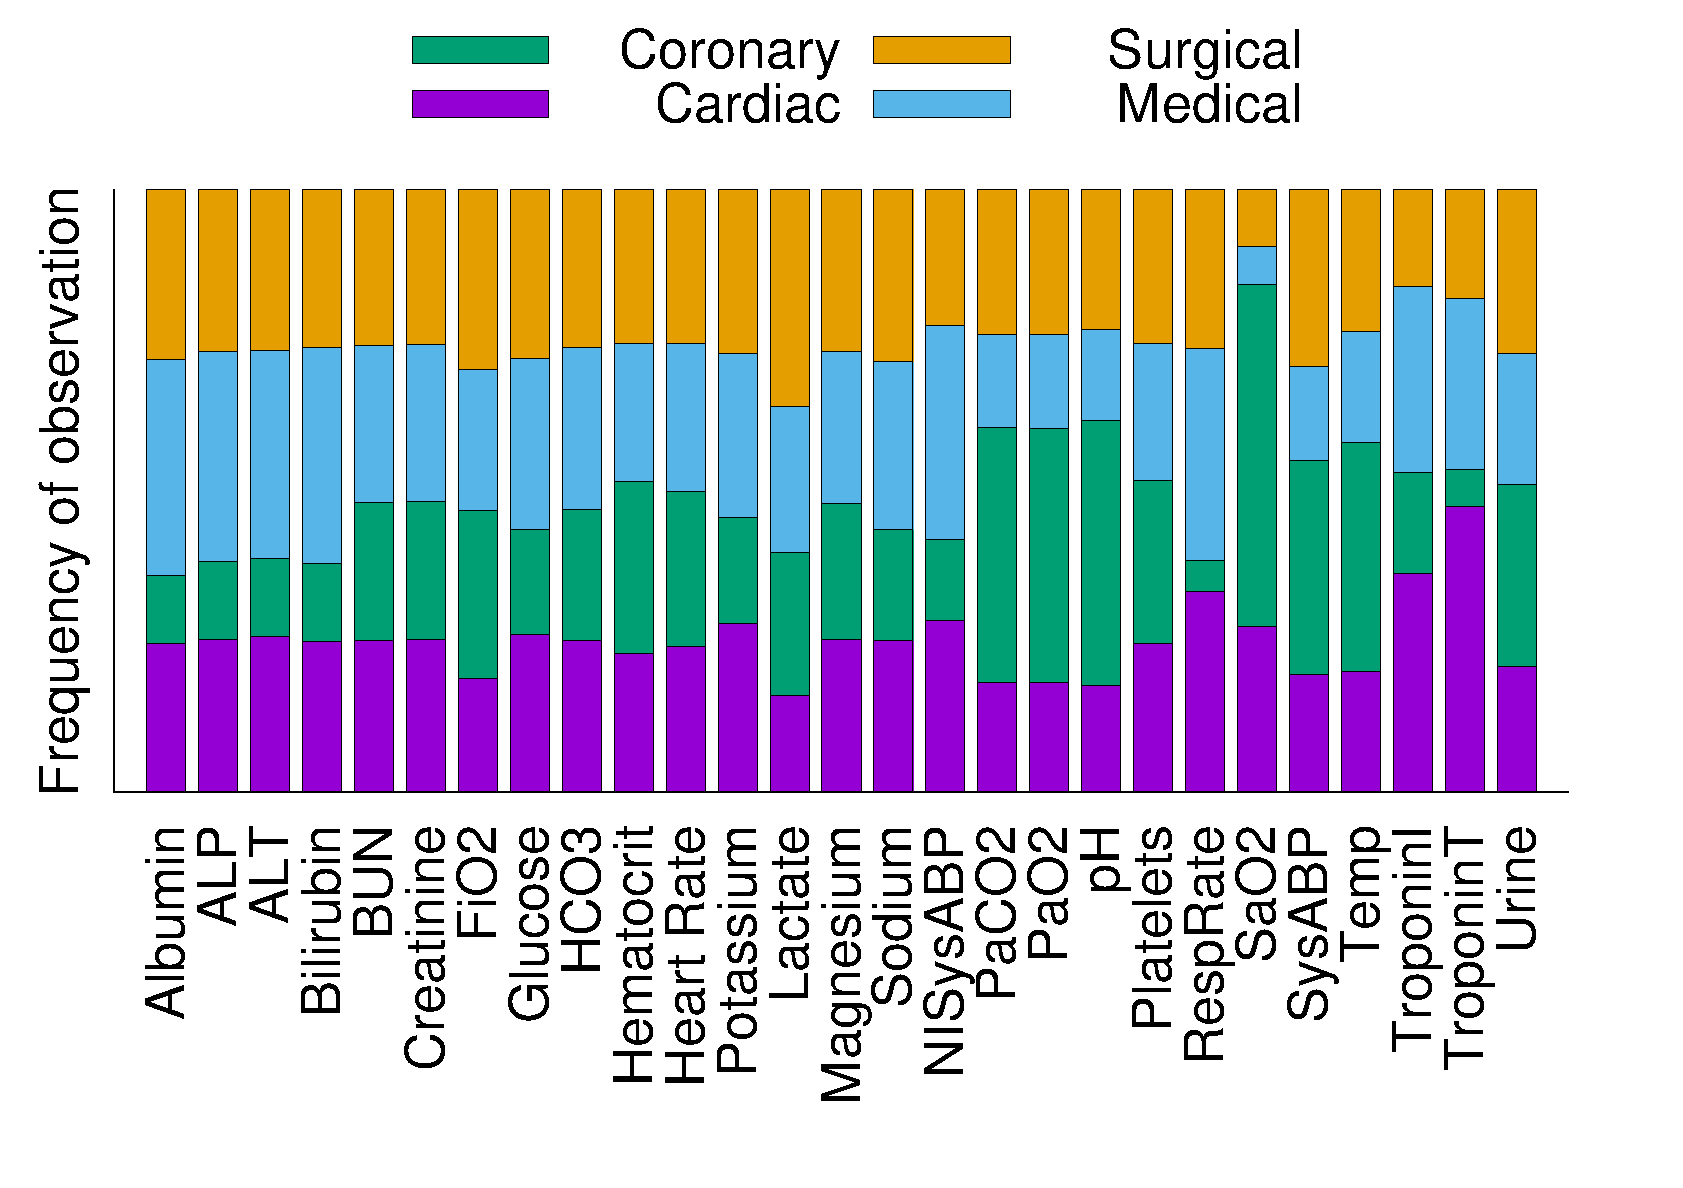
\includegraphics[width=1.06\linewidth]{figs/fobs}
	\end{center}
	\caption{(Color online) Relative frequency in which physiological parameters are measured in different ICU domains.}
	\label{fig:freq}
\end{figure}

\subsection{Network Architecture}

In this section we introduce the deep model architectures we evaluated to perform mortality prediction, eventually selecting those with best results. We compared several architectures, from using only a Convolutional Neural Network ~\citep{nips} or recurrent layer, to combining both, and adding intermediate layers, such as Dropout layers. Convolutional and recurrent components offer a complementary perspective of the patient condition, as follows: the convolutional layer emphasizes the local interaction between physiological parameters, while the recurrent layer is designed to capture long range information and forget unimportant local information. 

Our first model was a single recurrent layer, more specifically a LSTM layer that sought to capture the tendencies between the patient states each time. Long-Short Term Memories are largely used in time-dependent problems, because of its great ability to deal with series data, so its a natural choice in this case. As our patient can be understood as a series of points moving in a high dimensional space, the LSTM will be able to create a representation based on this movement, which is then used to perform prediction, although it may overlook the feature codependency in a single time step.

We also tried a Convolution-only model, that captured the relationship between features on a single time period, and then treated all time periods as one. This approach is not as intuitive as the later, but shows a surprisingly better performance. Here we create several filters that combine the patient observations only locally, this is, it does not combine features across time. Alongside a Max Pooling layer, the model extracts some information about risk regions in the patient's feature space over this local combination, and finally, all this information is flattened into a single vector that is the patients representation, then used to predict his outcome. Although this method does not explicit create a representation based on the patient time series, by creating a flatting representation with all the time steps we are also encapsulating time information.

Finally, we have the model that employs a CNN layer followed by a max-pooling layer, thus extracting correlations between physiological parameters measured in the same time period and exploring their simultaneous effects. For instance, it may find that if both temperature and heart rate are high on the same time period, the odds of survival decrease. In a complementary way, the recurrent layer (LSTM) is devoted to learn how changes in observations for a patient affect the corresponding outcome. Intuitively, the recurrent layer captures temporal dependencies, enabling the estimation of patient progress from the current patient state. For instance, if the heart rate was low at the beginning of the stay and then become very high, then the odds of survival decrease. Finally, a dense layer takes the output of the recurrent layer and predicts the patient outcome. This model is shown in~Figure~\ref{fig:arch}.

% \begin{figure}[htb]
\centering
%\begin{psmatrix}[mnode=r,colsep=0.1,rowsep=0.3]
$\psmatrix[mnode=r,colsep=0.1,rowsep=0.3]
&[name=a1]\footnotesize{<A_1,o_1>} && [name=c1] \footnotesize{<A_2,o_2>} &\ldots& [name=e1] \footnotesize{<A_{t-1},o_{t-1}>} && [name=g1] \footnotesize{<A_t,o_t>}\\[0pt]
& & & & & & &\\[0pt]
&[name=a2] \myx{\mbox{~\footnotesize{CNN}~}} & & [name=c2] \myx{\mbox{~\footnotesize{CNN}~}} & \ldots & [name=e2] \myx{\mbox{~\footnotesize{CNN}~}}& & [name=g2] \myx{\mbox{~\footnotesize{CNN}~}}\\[0pt]
& & & & & & &\\[0pt]
&[name=a3] \mybox{\mbox{\footnotesize{LSTM}}} & & [name=c3] \mybox{\mbox{\footnotesize{LSTM}}} & [name=x] \ldots & [name=e3] \mybox{\mbox{\footnotesize{LSTM}}}& & [name=g3] \mybox{\mbox{\footnotesize{LSTM}}}\\[0pt]
& & & & & & &\\[0pt]
& [name=a4] & & [name=c4] & & [name=e4] & & [name=g4]\\[0pt]
 && [name=a] && && [name=b]
\endpsmatrix $
\psset{nodesep=3pt,arrows=->}

\ncline{->}{a}{b}
\ncput*{\footnotesize{dynamic predictions}}
\ncline{->}{a1}{a2}
\ncline{->}{a2}{a3}
\ncline{->}{a3}{a4}
\ncput*{\footnotesize{Dense}}
\ncline{->}{c1}{c2}
\ncline{->}{c2}{c3}
\ncline{->}{c3}{c4}
\ncput*{\footnotesize{Dense}}
\ncline{->}{e1}{e2}
\ncline{->}{e2}{e3}
\ncline{->}{e3}{e4}
\ncput*{\footnotesize{Dense}}
\ncline{->}{g1}{g2}
\ncline{->}{g2}{g3}
\ncline{->}{g3}{g4}
\ncput*{\footnotesize{Dense}}
\nccurve[angleA=45,angleB=90]{a3}{c3}
\nccurve[angleA=45,angleB=90,linestyle=dashed]{c3}{e3}
\nccurve[angleA=45,angleB=90]{e3}{g3}
%\end{psmatrix}
\caption{Network architecture for predicting patient outcomes over time. Each convolutional (CNN) layer is followed by a LSTM layer and different feature transference approaches are designed using this architecture.}
\label{fig:arch}
\end{figure}



Naturally, this is a high variance data, since all features come from measuring something as complex as a human being, which leads to the model quickly overfitting the training set. In order to prevent this, we applied several dropout layers \cite{srivastava2014dropout}, specifically after the input, max pooling and LSTM layers. A dropout layer will choose a random set of neuron each batch, and disable them during training. This will make the other neurons (that were not disabled) generalize more, simulating the effect of training multiple smaller networks and averaging them during test. We drop from 20 to 30 percent of all neurons on each layer. We also apply L2 regularization \cite{wager2013dropout} to the LSTM inner cell neurons and the fully connected layer at the end of the model. This regularization will force each neuron to keep their activation weights low, thus generalizing more. Our loss function was binary cross-entropy, because of its good performance for classification problems with two classes. This loss function is given in the following formula:
\begin{center}
	$ \ell(\lambda) = -\frac{1}{n} \sum_{i=1}^{n}[y_{i}log(p_{i}) + (1 - y_{i})log(1 - p_{i})] + \lambda\sum_{j=1}^{k}w_{j}^2 $
\end{center}
where $ \lambda $ is the set of weights, $ n $ is the number of samples in the batch, $ y_{i} $ is the true output of the ith patient, $ p_{i} $ is the predicted output for the ith patient, and $ k $ is the number of neurons to regularize.

The final component tested in the neural architecture was the activation function of each layer. For the other layers, a few activation functions were tried: 
\begin{description}
	\item \textbf{Linear} $ f(x) = x $
	\item \textbf{Sigmoid} $ f(x) = \frac{1}{1 + e^{-x}} $
	\item \textbf{Tanh} $ f(x) = \frac{e^{x} - e^{-x}}{e^{x} + e^{-x}} $
	\item \textbf{Rectifier Linear Unit (ReLU)} $ f(x) = max(0, x) $
	\item \textbf{Scaled Exponential Linear Unit (SELU)} $ f(x) = \lambda x $, if x > 0, $ \alpha e^x - \alpha $, otherwise 
\end{description}
being x the neuron output. Since this is a binary classification problem, ranged from 0 to 1, we chose to sustain a sigmoid activation on the output layer. This will scale any output to the (0, 1) interval. 

In order to choose a set of model parameters that perform well for this task, a hand tuning method was applied. This means that we manually executed tests with different parameter sets and chose the set that performed, making adjustments based on the output of previous executions. Those parameters include the number of neurons on each layer, activation functions (as mentioned above), regularization type and amount, dropout percentage, along with some layer-specific parameters, such as kernel size, for convolutional layers and pool size for max pooling layers. 

% Combining convolutional and recurrent structures have been investigated in prior work other than  (Donahue et al., 2015; Zuo et al., 2015; Sainath et al., 2015).

In summary, our models works by passing each observation through a spatial feature extractor and then the sequence model captures how the extracted spatial features are associated with patient outcomes over time.
Also, dropout operation is performed after each layer of the network.

As not all the descriptors and time-series were available for all records, we had to deal with the problem of missing values. If one variable (either a descriptor or a time-series) was never recorded for a given record, we used the approach called "imputation" and replaced its feature/s with value zero. Because of the normalization step, this approximately corresponds to replacing the missing raw variable with a measure of central tendency, which corresponds to the arithmetic mean for Gaussian-distributed variables and to the geometric mean for log-normal ones. In some cases, the time-series measurement were taken only in the first 24 h or only during the next 24 h. In this case, replacing with zero all the features related to the period with missing measurements could possibly create a non-existing improvement or deterioration trend. Instead, we duplicate the values from the available period, assuming stationarity conditions as default in absence of further measurements.

\subsection{Switch Layer}

%TODO falar da switch

Dado tem muita variabilidade, mas podem haver padroes dentro dos dados. Em um caso otimo, estes padroes casariam exatamente com as UTIs
A switch tenta correlacionar as features em um espaço vetorial denso para representar estes padroes. A representaçao criada eh usada pra escalonar o proprio dado
Baiscamente eh um classificador


\subsection{Feature Transferability}

Our goal is to train multi-domain models to predict patient outcomes over time, which is based on patient observations associated with multiple ICU domains. Although patients associated with a given ICU domain may be better represented by specific features, there still exist some common features that permeate all other ICU domains. 

%\vspace{0.05in}
%\noindent{\bf{Transference Approaches}} 
The main intuition that we exploit for feature transferability is that the features must eventually transition from general to specific along our model, and feature transferability drops significantly in higher layers with increasing domain discrepancy~\citep{bengio2}. In other words, the features computed in higher layers must depend %greatly 
strongly on a specific domain, and prediction effectiveness suffers if this domain is discrepant from the target domain. Since we are dealing with many domains simultaneously, we tested multiple transference approaches, which are detailed as follows:

\begin{description}
\item [A1:] No layer is kept frozen during fine-tuning, i.e., errors are back-propagated through the entire network during fine-tuning.
\item [A2:] Only the convolutional layer is kept frozen during fine-tuning.
\item [A3:] Convolutional and LSTM layers are kept frozen during fine-tuning, i.e., errors are back-propagated only thought the fully-connected layers during fine-tuning.
\item [A4:] Only the convolutional layer is kept frozen during fine-tuning and other layers have their weights randomly initialized for fine-tuning.
\item [A5:] Convolutional and LSTM layers are kept frozen during fine-tuning and weights in fully-connected layers are randomly initialized for fine-tuning.
\end{description}


\section{Application}

Here we will present some ways of how a mortality prediction model can improve the work of medical doctors, helping them in their decisions.

%TODO predicao real time, pelo numero de pacientes e heatmaps

\section{Experiments}

In this section, we present the data we used to evaluate our multi-domain model for mortality prediction over time. Then, we discuss our evaluation procedure and report the results of our multi-domain model. In particular, our experiments aim to answer the following research questions:

\begin{description}
\item [RQ1:] Does domain adaptation improve mortality prediction? Do models that are specific to each ICU domain improve the state-of-the-art models for mortality prediction?
\item [RQ2:] Which feature transference approach is more appropriate to each ICU domain?
\item [RQ3:] How accurate are dynamic predictions?
\item [RQ4:] How meaningful are the mortality risk spaces created from patient trajectories?
\end{description}

\subsection{Baselines}

We considered the following methods in order to provide baseline comparison:

\begin{itemize}
\item Traditional classifiers: Support Vector Machines (SVM), Random Forest (RF), Logistic Regression (LR), Linear Discriminant Analysis (LDA), Quadratic Discriminant Analysis (QDA) and AdaBoost. The main objective of using these baselines is to compare our model with shallow models.
\item Training on Target (TT): A CNN$-$LSTM model is trained using only the target domain data. No source domain data is used. The main objective of using this baseline is to assess the benefits of different feature transference approaches.
\item Deep architecture~\citep{kdd}: A deep network that uses prior-based regularization. The main objective of using this baseline is to compare our model with state-of-the-art results on the PhysioNet data.
\end{itemize}

\subsection{Setup}

The measure used to evaluate the effectiveness of our models is the standard Area Under the ROC Curve (AUC), as adopted by~\citet{kdd}. Like~\citet{bayes}, we use five-fold cross validation and relevant hyper-parameters were found using a further internal cross-validation. The results reported are the average of the five runs and are used to assess the overall performance of the models. To ensure the relevance of the results, we assess the statistical significance of our measurements by means of a pairwise t-test~\citep{t-test} with p$-$value $\le 0.05$. Hereinafter, we refer to our model as CNN$-$LSTM.